\chapter{Discussion}\label{ch:overall}\label{ch:futurework}
\graphicspath{{../Figures/70-overall/}{figs/70-overall/}}

\section{Overview}\label{sec:foundation}

The research program connects two goals: using biology to improve robots and using biomimetic robots to investigate biology. Actuator mechanics and neural control must be considered together if a legged robot is to adapt to uneven terrain, disturbances, and changing loads. A sufficiently characterized robot also permits controlled changes to mechanics and sensory pathways that would be impractical or unethical in human experiments. Prosthetic and orthotic devices provide a further application of the resulting design and control knowledge.

This dissertation advances that program through four contributions: BPA force characterization, isometric joint-torque design factors, the Sensory Afferent Database, and tools for neuromechanical experiments. They address different sources of uncertainty between a proposed biological mechanism and a robotic test. The force and torque models support first-pass static sizing of the tested actuator and knee configurations; the database connects controller choices to published evidence; and the simulation tools make the resulting coupled systems available for controlled evaluation. Figure~\ref{fig:design_workflow} places these contributions within the broader development process.

\begin{figure}[htbp]
\centering
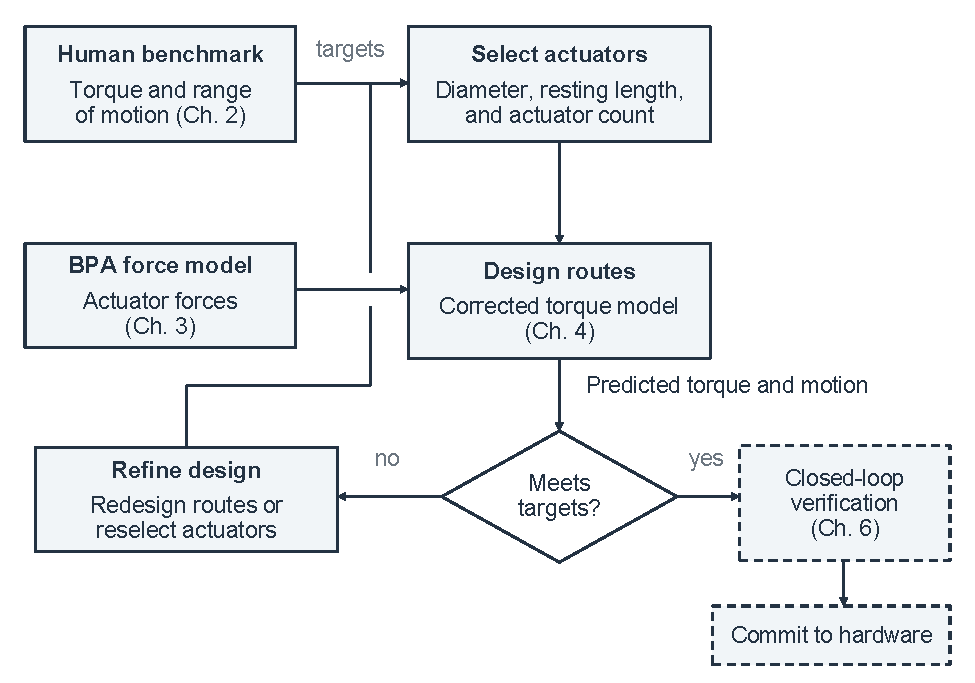
\includegraphics[width=\textwidth]{design_workflow.pdf}
\caption[The first-pass design workflow the enablers make possible]{Proposed workflow connecting human torque targets, BPA characterization, route design, neuromechanical simulation, and hardware development.}
\label{fig:design_workflow}
\end{figure}

\section{Research Contributions and Future Work}

\subsection{BPA Actuator Characterization}

Chapter~\ref{ch:muscles} establishes that the maximum isometric force of Festo BPAs depends on resting length, a design variable not represented adequately by the manufacturer's tool or the compared force models. The resting-length-dependent maximum-force model and three-coefficient nondimensional force surface provide a basis for selecting actuator length and predicting force across the measured contractions and pressures. This closes an actuator-sizing gap; it does not identify the complete dynamic behavior of a pressurized actuator.

\subsubsection{Future Work}\label{sec:fw_bpa}

The maximum-contraction function remains a useful next target. A predictive relationship between $\varepsilon_{620}$ and resting length was not established, so each actuator's free contraction must still be measured. Tests across product batches and the \qtylist{10;20;40}{\mm} diameters could distinguish a repeatable length dependence from batch variation. The characterized \qty{20}{\mm} actuators came from a single batch.

Dynamic characterization should distinguish active pressurized-braid force, passive resistance, and contraction dynamics. Biological muscle models provide a useful organizational framework for these components \citep{thelen_adjustment_2003,millard_flexing_2013}; Appendix~\ref{app:muscle_calcs} gives their constitutive relations. Constant-speed, constant-load, and constant-pressure experiments would extend the isometric measurements. The pressure--force model of \citet{elzein_pressure_2025} supplies a complementary starting point for pulse-modulated actuation.

Tensile tests with the Onyx and aluminum end caps, under pressurized and unpressurized conditions, could test the proposed end-effect explanation for resting-length-dependent force. A finite-element model of the rubber layers, crossed aramid braid, end constraints, and contact interfaces would connect that explanation to the construction described in the Festo patent literature \citep{festo_2026}. The proposed geometry in Figure~\ref{fig:bpa_construction} provides a starting point for comparing predicted deformation with measured behavior.

\begin{figure}[htbp]
\centering
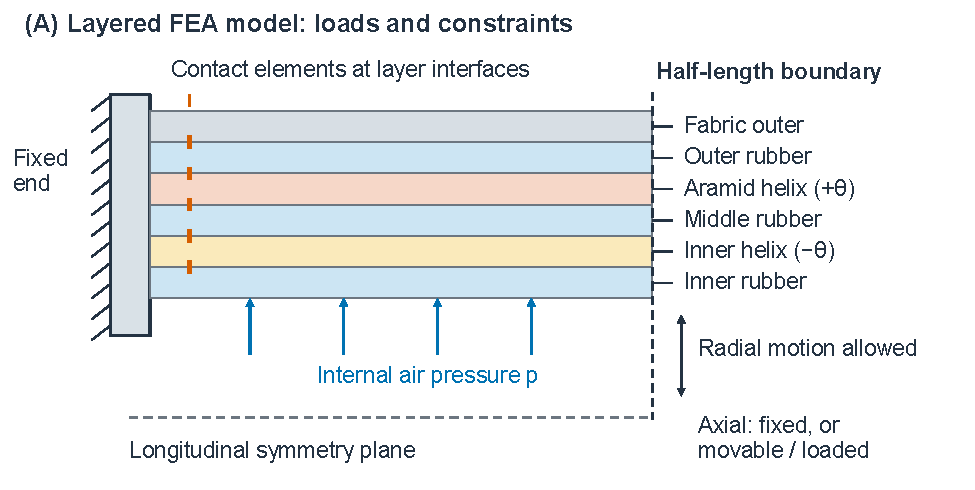
\includegraphics[width=0.94\textwidth]{bpa_construction.pdf}\par\smallskip
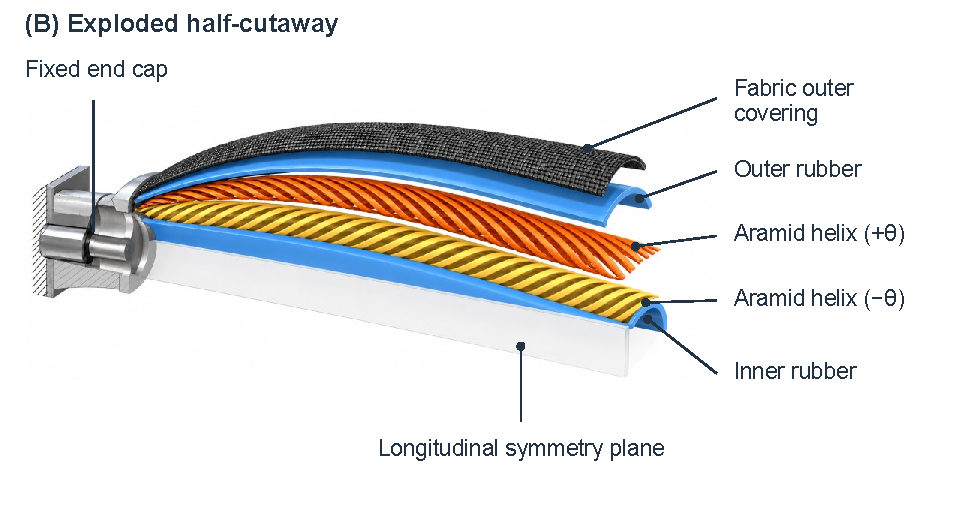
\includegraphics[width=0.94\textwidth]{bpa_exploded_cutaway.pdf}
\caption{Proposed layered BPA finite-element model: contact and boundary conditions (A), and illustrative material cutaway (B). Geometry and layer spacing are schematic; the middle rubber layer is separated only in A.}
\label{fig:bpa_construction}
\end{figure}

\subsection{Isometric Joint Design Factors}

Chapter~\ref{ch:torque} shows why actuator force and rigid-body moment arms alone are insufficient to predict the tested knee torques. Length offsets, effective series compliance, and wrapping-induced loss of usable actuator length affect the transmitted force. The identified corrections improve prediction across the tested configurations and support the redesigned flexor and extensor routes. Their measured capacity meets or exceeds the selected human-muscle references at the tested knee angles. These results extend the earlier attachment-placement work \citep{bolen_bipedal_2019,bolen_determination_2019,morrow_optimization_2020} from geometric prediction toward experimentally informed joint design.

\subsubsection{Future Work}\label{sec:fw_routing}

The next mechanical questions concern transfer and packaging. The staggered flexor paths need physical clearance, load-sharing, and off-axis-load checks before extension to a complete leg. Reeved routes require space as well as sufficient torque, and the broader route search still contains incomplete configurations (Appendix~\ref{sec:app_routing_extensions}). A cam or artificial patella offers another way to control moment arm and protect an actuator from joint contact, but friction and contact transitions must be included when assessing such a design. The cam result supports further investigation; it does not establish the performance of an artificial patella.

The correction set also leaves a mechanical hypothesis to test: an additional force-path stiffness, $\chi_{4}$, may explain effects presently absorbed into the orientation-dependent stiffness pair. This can be investigated through the existing identification framework without treating the current effective stiffnesses as literal bracket material properties.

Controlled-speed and controlled-load knee tests would extend the static capacity measurements to movement. Loading--unloading sequences would characterize hysteresis, and pressure-step tests would characterize the pneumatic response. A torque-controlled motor and a less compliant loading connection would reduce winch slack and permit these tests on the existing rig. These experiments would establish where the isometric model remains useful and where velocity dependence, damping, or pressure regulation needs an additional model.

\subsection{Sensory Afferent Database}

Chapter~\ref{ch:database} addresses a different gap: selecting sensory feedback requires evidence distributed across animal studies, human studies, and computational models. SADb makes that evidence searchable through curation notes, linked records, classifications, and citation neighborhoods. It supports tracing a proposed pathway to its source and comparing the conditions under which a response was observed. The contribution is the research collection and its navigation tools, rather than a claim that every record is fully classified or every proposed feedback rule transfers directly to a robot.

\subsubsection{Future Work}\label{sec:fw_database}

The implemented monthly literature watch produces candidate shortlists for manual curation (Section~\ref{sec:sadb_methods}). Continued work should complete useful classifications and connect model assumptions to the primary experiments that support them. Each pathway record should identify its sensory signal, connection sign, task dependence, and source; each model record should identify the pathways it implements. Search and summarization tools can assist this process, while inclusion and interpretation remain research judgments \citep{bolen_using_2024}.

Vestibular, visual, and multisensory contributions to posture provide useful areas for expansion. Better links between their experimental conditions and modeled mechanisms would support the sensory extensions below. Source availability should be checked during curation; records whose sources cannot be located should be removed from the working research base rather than treated as verified evidence. This is a curation rule, not a claim that a particular number of existing records has already failed that check.

\subsection{SNS Tools and Neuromechanical Experiments}

Chapter~\ref{ch:sns} begins with a controller-transfer problem: placing an existing neural controller on a different biomechanical model and tuning it by hand produced stepping-like motion in the air, but not walking. That experience motivated tools for constructing, inspecting, tuning, and comparing more complex neural--mechanical systems. The implemented models, graphical blocks, simulation interfaces, and curriculum support those tasks. Matched-input tests establish selected implementation agreement, reflex demonstrations show corrective feedback, and fixed-controller pathway removal tests sensory dependence in supported stepping.

The later virtual-harness-assisted evaluations establish coupled balance and locomotor behaviors while retaining their stated support conditions. Human-model stepping persists after removal of externally supplied neural drive, in place under the support rig; the robot model progresses under its harness with reduced drive (Section~\ref{sec:sns_controller_comparison}). Neural-drive dependence and mechanical-support dependence are different experimental questions. The balance-platform studies provide a separate hardware precedent for BPA-actuated balance with pseudo-vestibular feedback \citep{bolen_balance_2024,bolen_selfbalancing_2024,bolen_selfbalancing_srs_2024}.

\subsubsection{Future Work}\label{sec:fw_pipeline}\label{sec:fw_cpg}

The next controller-transfer experiments should compare defined neural and mechanical configurations under matched stimuli and tuning conditions. Stimulation at the rhythm-generator, pattern-formation, and motoneuron layers can distinguish resetting the neural clock from suppressing motor output (Section~\ref{sec:app_layer_stimulus}). Physiological and modeling studies supply reference phenomena \citep{selionov_tonic_2009,rybak_modelling_2006,markin_afferent_2010,shevtsova_modeling_2016}. Pathway additions and removals should retain the other settings so that an observed change can be associated with the intervention. Spiking and non-spiking controllers require the same care when comparing their responses.

\paragraph{Sensory and Higher-Level Control}\label{sec:fw_senses}

Vestibular feedback could extend the balance-platform work using estimates of body orientation and angular velocity \citep{hilts_dynamic_2019,bolen_balance_2024}. Visual measurements could complement those estimates and help correct inertial drift. Their integration should follow the task-dependent sensory weighting established in the relevant literature, rather than assuming that one channel always dominates \citep{akay_relative_2021}. Figure~\ref{fig:sensorium_hierarchy} separates these proposed additions from the implemented spinal and body-model components.

Cerebellar and basal-ganglia models offer further questions about adaptation, coordination, and action selection. Multilevel synthetic nervous systems for insect-like legs \citep{grummer_multilevel_2024} and cortico-cerebellar-spinal models of adaptive step length \citep{chen_corticocerebellar_2025} provide starting points. Such extensions should be evaluated for a defined change in behavior, rather than added solely to make the controller more anatomically elaborate.

\begin{figure}[htbp]
\centering
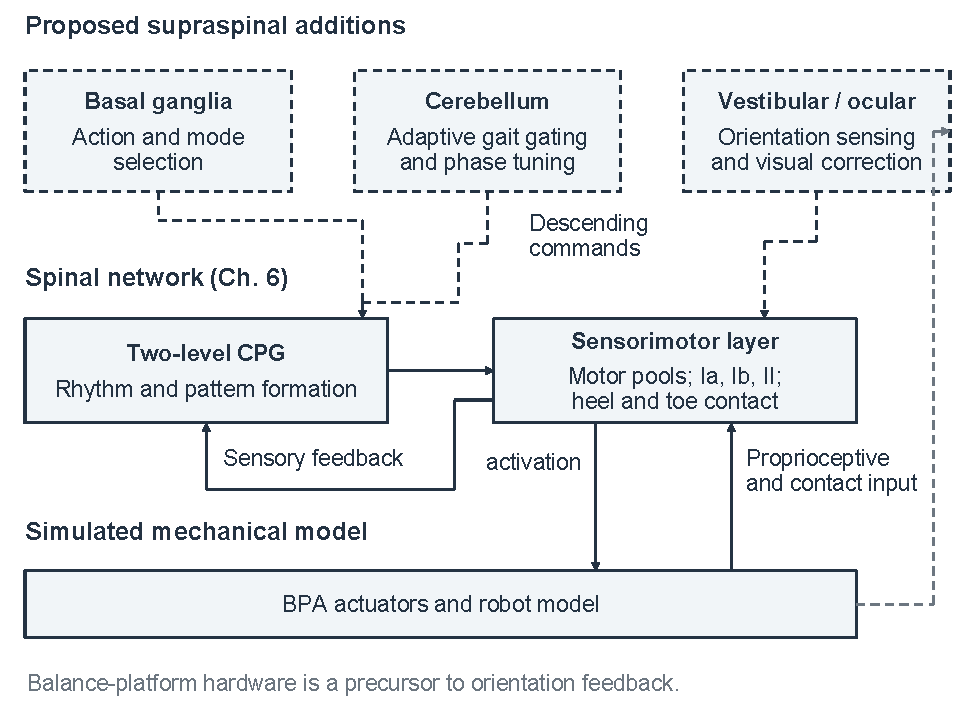
\includegraphics[width=0.96\textwidth]{sensorium_hierarchy.pdf}
\caption[Control stack with the planned supraspinal additions]{Control hierarchy connecting spinal pathways and the BPA-actuated model to proposed supraspinal and sensory extensions. Dashed elements indicate future work.}
\label{fig:sensorium_hierarchy}
\end{figure}

\paragraph{Hardware Transfer}\label{sec:fw_hardware}

Figure~\ref{fig:pipeline} places the implemented simulation interfaces within the proposed hardware workflow. The model-construction and controller-editing routes are detailed in Figure~\ref{fig:simulation_workflow}. Computer-in-the-loop testing would connect the actual embedded controller to the simulated robot before physical deployment; valve-control interfaces and treadmill deployment remain integration tasks.

\begin{figure}[htbp]
\centering
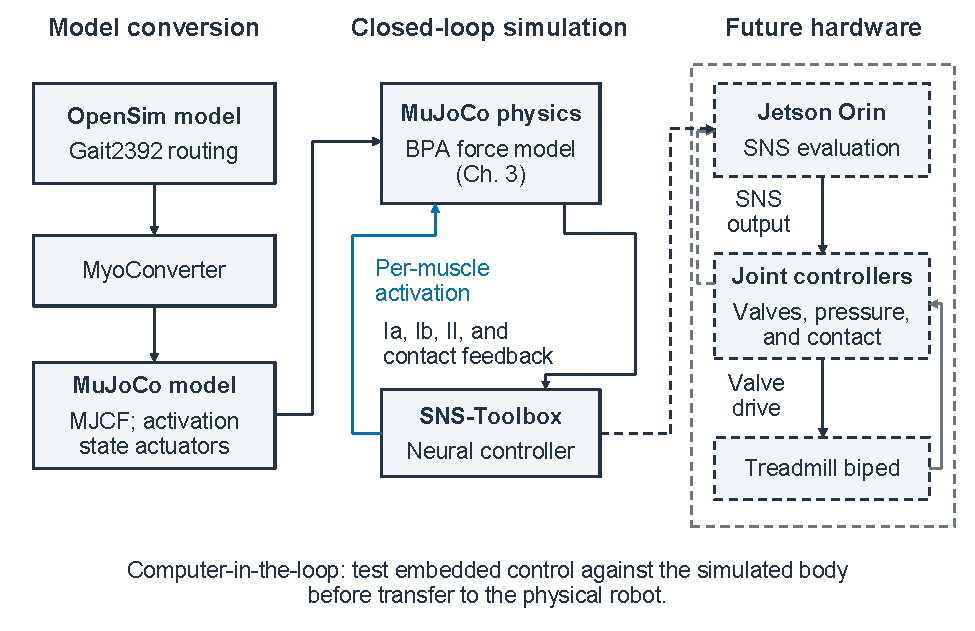
\includegraphics[width=\textwidth]{pipeline.pdf}
\caption[Simulation-to-hardware workflow]{Model conversion, closed-loop simulation, and proposed hardware deployment. Simulation interfaces exchange actuator commands and afferent signals. The embedded valve-control and network-evaluation system and treadmill deployment are future work.}
\label{fig:pipeline}
\end{figure}

The hardware objective is low-latency joint control on Teensy-class microcontrollers and neural-network evaluation on an NVIDIA Jetson Orin. Encoders, strain gauges, pressure sensors, contact sensors, and IMUs would supply the sensory channels. Length and velocity estimates are needed for Ia/II feedback, while Ib force estimates must account for actuator length and loading direction. The static force and torque maps could supply feedforward commands, complemented by pressure--force dynamics \citep{elzein_pressure_2025}.

Physical PAM-biped control \citep{li_controller_2024} and the transfer of Muscle Mutt's SNS controller from MuJoCo to hardware \citep{lutz_mechanical_2025} support further investigation of that route. They do not validate the present biped. Each new body model, actuator configuration, and controller combination needs its own geometry, interface, and behavioral checks.

\paragraph{Dynamic Whole-Body Maneuvers}\label{sec:fw_kickflip}

Beyond steady locomotion, the program aims at gait transitions, reactive balance, and dynamic whole-body maneuvers. My longer-term aspiration is a robot that can perform a kickflip, requiring coordinated extension, aerial orientation, and controlled landing. That goal connects the actuator and routing questions to contact sensing, spinal coordination, vestibular estimation, and higher-level adaptation.

\section{From Design Tools to Neuromechanical Experiments}

Together, the four contributions connect mechanical designs and neural hypotheses to controlled tests. Dynamic characterization, sensory integration, and hardware transfer could extend this foundation toward autonomous robots and more informative models of biology. Chapter~\ref{ch:conclusion} summarizes the established findings and their implications.
